\documentclass[12pt]{article}
\usepackage[a4paper, total={7.5in, 11in}]{geometry}
%\usepackage{array}
\usepackage{graphicx, subfig, wrapfig, fancyhdr, lastpage, multicol ,color, pgfplots,circuitikz}
\newcommand\headerMe[2]{\noindent{}#1\hfill#2}
\usepackage[mathscr]{euscript}
\usepackage{tabularray}

\setlength{\columnseprule}{1pt}
\def\columnseprulecolor{\color{blue}}


\pagestyle{fancy}
\fancyhf{}

\cfoot{ \vspace{-0.8cm}\em{Page \thepage \hspace{1pt} / \pageref{LastPage}}}
\begin{document}

\headerMe{Royaume du Maroc}{année scolaire \emph{2024-2025}}\\
\headerMe{Ministère de l'Éducation nationale, }{  Professeur :\emph{Zakaria Haouzan}}\\
\headerMe{du Préscolaire et des Sports}{Établissement : \emph{Lycée SKHOR qualifiant}}\\

\begin{center}
  \vspace{-1cm}
Devoir Surveillé  N°1 - semestre 02 \\
    2ème année baccalauréat Sciences Mathématiques\\
Durée 2h00
\\
    \vspace{-0.2cm}
\hrulefill
\Large{Chimie 7pts/42min}
\hrulefill\\


\end{center}
%end Headerss------------------------
%__________________Chimie ______________________-
%%%%%%%+_+_+_+_+_+_+_+_+_Partie1

\vspace{-1cm}
 \section*{ Étude d’une pile d’Argent-Cuivre \dotfill(7pts) }
On considère une pile cuivre-argent réalisée à partir de deux lames de masse $m = 10,00$ g chacune. Les solutions aqueuses de nitrate d'argent et de sulfate de cuivre utilisées sont des solutions de concentration apportée $C = 0,1$ mol.L$^{-1}$. Leur volume individuel est $V = 50,0$ mL. 

On donne :
\[
M({Cu}) = 63,5  g.mol^{-1}, \quad M(Ag) = 107,9  g.mol^{-1}
\]
Cette pile débite dans une résistance $R = 4,6 \, \Omega$. Un voltmètre placé aux bornes de cette pile indique :
\[
U_{{Cu/Ag}} = -0,46 { V}.
\]

\begin{enumerate}
  \item  Préciser le pôle positif de cette pile. \dotfill(1pt)

  \item  Donner le schéma conventionnel de cette pile.\dotfill(1pt)

  \item  Écrire les deux demi-équations électroniques des réactions modélisant les transformations ayant lieu aux interfaces métal-solution puis en déduire l'équation globale de la réaction.\dotfill(1pt)

  \item Citer les deux rôles du pont salin.\dotfill(0,5pt)

  \item On suppose que cette pile débite un courant continu d'intensité constante $I = 100$ mA pendant une durée $\Delta t = 10$ min 30 s. Au bout de cette durée déterminer :

    \begin{itemize}
        \item[(a)] La quantité d'électricité débitée par la pile.\dotfill(0,5pt)
        \item[(b)] L'avancement de la réaction.\dotfill(0,5pt)
        \item[(c)] Le taux d’avancement.\dotfill (0,5pt)
        \item[(d)] La masse de l’électrode d’argent. \dotfill(0,5pt)
        \item[(e)] La concentration des ions cuivre. \dotfill(0,5pt)
    \end{itemize}


  \item Sachant que la constante de la réaction vaut $K = 10^{35}$, calculer la capacité de cette pile en mA.h.(1pt)


\end{enumerate}

%\hrulefill
%\Large{Physique 13pts/78min}
%\hrulefill\\
\begin{center}
    %\vspace{.60cm}
\hrulefill
\Large{Physique 13pts}
\hrulefill\\
    \emph{Les deux parties sont indépendantes}
\end{center}


\section*{Partie 1:Autour de l’oscillateur LC \dotfill(3pts) }

\begin{wrapfigure}[1]{r}{0.25\textwidth}
  \vspace{-1cm}
\includegraphics[width=1\linewidth]{./lc.png} 
\end{wrapfigure}

On réalise le montage électrique représenté dans la figure 1, formé de :
\begin{itemize}
    \item Un générateur $G$ idéal de tension de force électromotrice $E = 12V$ ;
    \item Une bobine d’inductance $L$ et de résistance négligeable.
    \item Deux condensateurs $(C_1)$ et $(C_2)$ de capacités respectives $C_1 = 3 \mu F$ et $C_2 = 0,5 C_1$ ;

\end{itemize}

\subsection*{1. Chargement des condensateurs}
    - On place l’interrupteur $K$ dans la position (1), alors les deux condensateurs se chargent instantanément. Soit $U_1$ la tension aux bornes du condensateur $(C_1)$ et $U_2$ la tension aux bornes du condensateur $(C_2)$.

\begin{enumerate}
  \item[1.1] Calculer $U_1$ et $U_2$.\dotfill(0,25pt)
  \item[1.2] Soit $E_1$ l’énergie électrique emmagasinée dans le condensateur $(C_1)$ et $E_2$ l’énergie électrique emmagasinée dans le condensateur $(C_2)$. Montrer que $E_2 = 2E_1$.\dotfill(0.5pt)
\end{enumerate}

\begin{center}
 
  \vspace{-0.4cm}

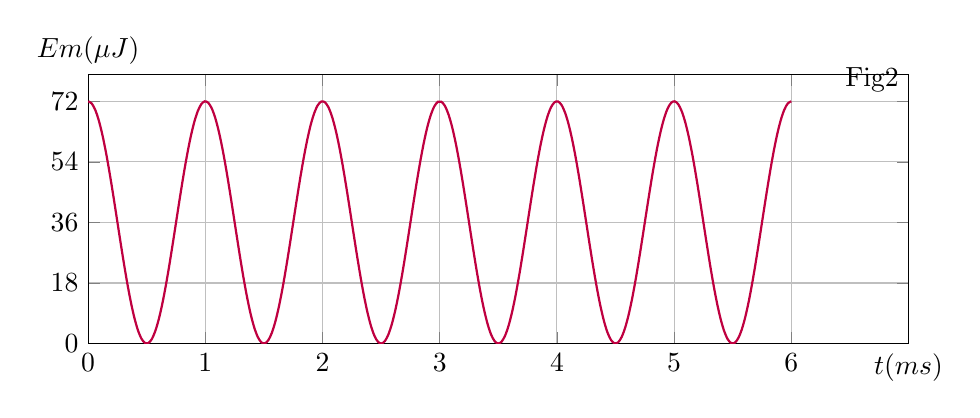
\begin{tikzpicture}
\begin{axis}[
    xlabel={$t(ms)$},
    ylabel={$Em(\mu J)$},
    xmin=0, xmax=7,
    ymin=0, ymax=80,
    xtick={0,1,2,3,4,5,6},
    ytick={0,18,36,54,72},
    grid=both,
    minor grid style={gray!25},
    major grid style={gray!50},
    width=12cm,
    height=5cm,
    title={Fig2},
    title style={anchor=north east, at={(1,1)}},
    every axis x label/.style={at={(axis description cs:1,0)},anchor=north},
    every axis y label/.style={at={(axis description cs:0,1)},anchor=south},
]
\addplot[
    domain=0:6,
    samples=200,
    smooth,
    thick,
    purple,
    ] {72*sin(deg(pi*x-pi/2))*sin(deg(pi*x-pi/2))};
\end{axis}
\end{tikzpicture}

\end{center}

\vspace{-1cm}
\subsection*{2. Déchargement à travers la bobine}
     On bascule à l’instant $t = 0$ l’interrupteur $K$ dans la position (2), alors les deux condensateurs se déchargent à travers la bobine. La figure (2) représente l’évolution temporelle de l’énergie magnétique $E_m$ emmagasinée dans la bobine.

     \begin{enumerate}
       \item[2.1] Montrer que la tension $u_c$ vérifie l'équation différentielle :
$    \frac{d^2 u_c}{dt^2} + \frac{1}{LC} u_c = 0$\dotfill(0.25pt)

    \item[2.2] Trouver l’expression de la période propre $T_0$ en fonction de $L$ et $C_1$ pour que la solution de l’équation différentielle soit:
      $
    u_c(t) = U_{{max}} \cos \left(\omega_0 t + \phi \right)
   $ \dotfill(0.5pt)
 \item[2.3] En déduire que $L = 0,4H$ en prenant $\pi^2 = 10$. \dotfill(0.5pt)    
    \item[2.4] Montrer que l’énergie totale $E_T$ emmagasinée dans le circuit reste constante au cours du temps avec    $
    E_T = \frac{1}{2} \left( C_{{eq}} u^2 + L i^2 \right)
   $ \dotfill(0.5pt)

    \item[2.5] Déterminer à l’aide du graphe (fig2) la valeur de l’énergie emmagasinée dans le condensateur équivalent à l’instant $t = 2ms$.\dotfill(0.5pt)

     \end{enumerate}


\section*{Partie 2 : Etude du dipôle RLC et la résonance d’intensité  \dotfill(4pts) }

\begin{wrapfigure}[14]{r}{0.4\textwidth}
  \vspace{-1.5cm} 
\begin{center}
  \begin{circuitikz}[scale=0.7]
    % Left voltage source (GBF)
    \draw (0,0) to[sV, l=GBF] (0,3);
    
    % Top horizontal line with resistor and inductor
    \draw (0,3) -- (1,3);
    \draw (1,3) to[R, l=R] (3,3);
    \draw (3,3) to[L, l=$L_r$] (5,3);
    
    % Right vertical line with capacitor
    \draw (5,3) to[C, l=C] (5,0);
    
    % Bottom horizontal line with ammeter
    \draw (5,0) -- (3,0);
    \draw (3,0) to[ammeter, l=A] (1,0);
    \draw (1,0) -- (0,0);
    
    % Figure caption
    \node at (2.5,-1) {Figure 1.};
\end{circuitikz}
\end{center}
  \vspace{-2cm}
\begin{center}
  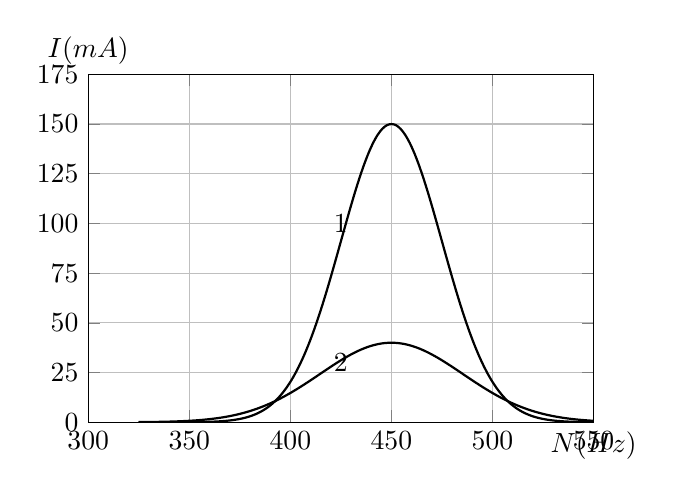
\begin{tikzpicture}
\begin{axis}[
    xlabel={$N(Hz)$},
    ylabel={$I(mA)$},
    xmin=300, xmax=550,
    ymin=0, ymax=175,
    xtick={300, 350, 400, 450, 500, 550},
    ytick={0, 25, 50, 75, 100, 125, 150, 175},
    grid=both,
    minor grid style={gray!25},
    major grid style={gray!50},
    width=8cm,
    height=6cm,
    every axis x label/.style={at={(axis description cs:1,0)},anchor=north},
    every axis y label/.style={at={(axis description cs:0,1)},anchor=south},
]

% First curve (higher peak)
\addplot[
    domain=325:550,
    samples=100,
    smooth,
    thick,
    ] {150*exp(-((x-450)^2)/1250)};
\node at (axis cs:425,100) {1};

% Second curve (lower peak)
\addplot[
    domain=325:550,
    samples=100,
    smooth,
    thick,
    ] {40*exp(-((x-450)^2)/2500)};
\node at (axis cs:425,30) {2};

\end{axis}
\end{tikzpicture}
\end{center}



\end{wrapfigure}


On étudie la résonance d’intensité d’un dipôle comprenant :
\begin{itemize}
    \item un résistor de résistance $R$ variable,
    \item une bobine d’inductance $L$ et de résistance $r$,
    \item un condensateur de capacité $C = 1\ \mu F$,
    \item un ampèremètre de résistance négligeable.
\end{itemize}

Ce circuit est alimenté par un générateur qui délivre une tension sinusoïdale de fréquence $N$ variable et de valeur efficace constante $U = 4,5V$ (figure 1).

La valeur de la résistance $R$ est ajustée de façon qu’elle prenne successivement les valeurs :
$R_1 = 20\ \Omega, \quad R_2 = 110\ \Omega$.
On fait varier la fréquence de la tension délivrée par le générateur, et pour chaque valeur de $N$, on relève l’intensité efficace $I$ du courant circulant dans le circuit, puis on trace la courbe $I = f(N)$ pour les deux valeurs de $R$ choisies. On obtient le graphique de la figure 2.

\begin{enumerate}
  \item À quelle résistance, $R_1$ ou $R_2$, correspond la courbe 1 ? Justifier la réponse.\dotfill(0.25pt)
  \item Déduire de la courbe 1 la fréquence de résonance du circuit.\dotfill(0.25pt)
  \item Que peut-on dire de l’influence de la valeur de la résistance du circuit sur la fréquence de résonance ?\dotfill(0.25pt)
  \item Déterminer l’inductance $L$ et la résistance $r$ de la bobine.\dotfill(0.5pt)
  \item Calculer la valeur de $Q$.\dotfill(0.5pt)
\end{enumerate}

On s’intéresse maintenant au phénomène de résonance d’intensité étudié à l’aide d’un oscilloscope, pour un circuit RLC analogue à celui représenté par la figure 1, avec les valeurs : $C_1 = 10\ \mu F, R_1 = 200\ \Omega,$.



\begin{center}
  
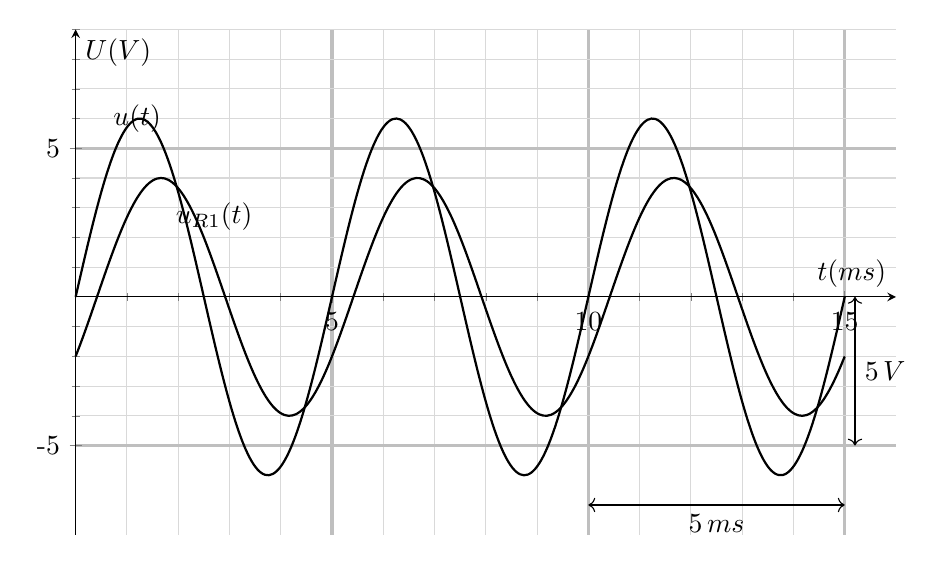
\begin{tikzpicture}
\begin{axis}[
    xlabel={$t(ms)$},
    ylabel={$U(V)$},
    xmin=0, xmax=16,
    ymin=-8, ymax=9,
    xtick={0,5,10,15},
    xticklabels={0,5,10,15},
    ytick={-5,0,5,10},
    yticklabels={-5,0,5},
    grid=both,
    minor tick num=4,
    minor grid style={gray!30},
    major grid style={gray!50, very thick},
    width=12cm,
    height=8cm,
    every axis x label/.style={at={(axis description cs:0.98,-0.02)},anchor=north west},
    every axis y label/.style={at={(axis description cs:-0.02,0.98)},anchor=south east},
    axis lines=middle,
    enlargelimits=false,
    clip=false,
]

% First curve - u(t)
\addplot[
    domain=0:15,
    samples=200,
    smooth,
    thick,
    black,
    ] {6*sin(deg(2*pi*x/5))};
\node[black] at (axis cs:1.2,6) {$u(t)$};

% Second curve - u_R(t)
\addplot[
    domain=0:15,
    samples=200,
    smooth,
    thick,
    black,
    ] {4*sin(deg(2*pi*x/5 - pi/6))};
  \node[black] at (axis cs:2.7,2.7) {$u_{R1}(t)$};

% Scale indicators
\draw[<->] (axis cs:10,-7) -- (axis cs:15,-7) node[midway,below] {$5\,ms$};
\draw[<->] (axis cs:15.2,-5) -- (axis cs:15.2,0) node[midway,right] {$5\,V$};

\end{axis}
\end{tikzpicture}

\end{center}


\begin{enumerate}
    \setcounter{enumi}{6}
    \item On modifie la fréquence $N$ de la tension délivrée par le générateur de manière à chercher la résonance d’intensité. Au cours de cette recherche, on observe pour une fréquence $N_1$ du générateur les courbes représentées ci-contre. Déterminer :
    \begin{enumerate}
      \item La valeur numérique de la fréquence $N_1$.\dotfill(0.25pt)
      \item Le déphasage $\varphi$ de $u(t)$ par rapport à $u_{R1}(t)$.\dotfill(0.5pt)
      \item Les valeurs maximales $U_m$ de $u(t)$ et $U_{Rm}$ de $u_R(t)$.\dotfill(0.5pt)
      \item En déduire la valeur de l’impédance $Z$ du circuit.\dotfill(0.25pt)
    \end{enumerate}
  \item Lorsque la résonance est atteinte, quelle particularité présentent les deux courbes ?\dotfill(0.75pt)
\end{enumerate}


\section*{Partie 2 :  Applications: Production d'ondes électromagnétiques et
communication \dotfill(6pts)}

\begin{wrapfigure}[6]{r}{0.3\textwidth}
	\vspace{-1.2cm}
\begin{center}
  \includegraphics[width=0.3\textwidth]{./ex_031.png}
\end{center}
\vspace{-0.9cm}
\caption{}
\end{wrapfigure}



\emph{Lors d’une communication, la voix est convertie en signal électrique par un microphone, grâce à un système de
conversion numérique et d’amplification. Le signal électrique est porté par une onde porteuse qui après
amplification est émise vers l’antenne la plus proche. L’antenne transmet le signal à une station base qui
l’envoie alors à une centrale, par ligne téléphonique conventionnelle ou par les ondes électromagnétiques.}
 \\De là sont acheminées les conversations vers le
téléphone du destinataire.

\section*{1.Émission d’une onde électromagnétique par un portable}

Les ondes électromagnétiques sont utilisées par la
télévision, La radio et les radars. Si bien que la gamme de
fréquence restant pour les portables sont de plus en plus
restreints : l’une d’entre elles s’étend de 900 à 1800 MHz.

\textbf{Données : }La célérité des ondes électromagnétiques
dans le vide et dans l’air : $c = 3,00.10^8 m.s^{-1}$; $1MHz =10^6Hz$.

  \begin{enumerate}
    \item  Calculer la durée que met une onde électromagnétique de fréquence $f=900MHz$ pour parcourir la distance $M_1M_2=1km$ séparant le téléphone et l’antenne, figure (1).\dotfill(0,25pt) 
    \item Que signifie l’expression \emph{l’air est un milieu dispersif pour les ondes électromagnétiques} ?\dotfill(0,25pt)
    \item On peut représenter la chaine d’émission par le schéma de la figure (3).En quel point A  ou B ou C de la figure (3) trouve-t-on L’onde porteuse ? Le signal modulant ? \dotfill(0,25pt)

  \end{enumerate}
\begin{center}
  \includegraphics[width=0.6\textwidth]{./ex_032.png}
\end{center}

\vspace{-1.4cm}
\section*{2.Modulation d’amplitude \dotfill }

\begin{wrapfigure}[10]{r}{0.3\textwidth}
	\vspace{-1.2cm}
\begin{center}
  \includegraphics[width=0.3\textwidth]{./ex_033.png}

  \includegraphics[width=0.3\textwidth]{./ex_034.png}
\end{center}
\end{wrapfigure}



Le circuit de modulation est constitué d’un composant nommé multiplieur
qui possède deux entrées E1 et E2 et une sortie S,

Pour simuler la modulation d’amplitude, on applique :
\begin{itemize}

	\item À l’entrée $E_1$ le signal $u_1(t)=u(t)+U_0$ dont $u(t)=U_mcos(2.\pi.f.t)$ est\\ le
signal modulant et $U_0$ tension continue de décalage .
\item À l’entrée $E_2$ le signal porteur $u_2(t)=v(t)=V_m.cos(2.\pi.F.t)$.
\item Le circuit intégré X donne une tension modulée proportionnelle
au produit des deux tensions, $s(t)$=$ k.u_1(t).u_2(t)$ où k est une
constante dépendant uniquement du circuit intégré . s(t) s’écrit
sous la forme : $s(t)$=$S_mcos(2.\pi.F.t)$.
\end{itemize}

\begin{enumerate}

    \setcounter{enumi}{3}
  \item Montrer que $S_m$,amplitude du signal modulé , peut se
mettre sous \\la forme $S_m = A.\big[m.cos(2.\pi.f.t)+1\big]$ en précisant
    l’expression du \\taux de modulation m et celle de la constante A .............(0,5pt)
  \item Le graphe représenté sur la figure (5) donne l’allure de la
tension \\modulée en fonction du temps. Déterminer à partir de ce
graphe .
\begin{enumerate}
  \item la fréquence F de l’onde porteuse .\dotfill(0,25pt)
  \item la fréquence $f$ de l’onde modulant .\dotfill(0,25pt)
  \item L’amplitude minimale $S_{m(min)}$ et l’amplitude maximale $S_{m(max)}$ du signal modulé.\dotfill(0,25pt)

\end{enumerate}
    \item Donner l’expression du taux de modulation (m) en fonction de $S_{m(min)}$ et $S_{m(max)}$. Calculer sa valeur.\dotfill(1pt)

    \item La modulation effectuée est-elle de bonne qualité ? Justifier. \dotfill(0,5pt)

    \item Pour une bonne réception du signal modulée, on utilise un
circuit bouchon(circuit d'accord) formé d'une bobine
d'inductance $L_0 = 60mH$ et de résistance négligeable et
deux condensateurs , montés en série, de capacité $C =10\mu.F$
    et $C_0$ .\underline{Déterminer la valeur de $C_0$?}. Tracer le disjoncteur (circuit d'accord) et expliquer le rôle de chaque étape ? \dotfill(2,5pt)

\end{enumerate}

\end{document}
